\section{MultiSearch Engine}

We call our new search algorithm within \astar a \emph{MultiSearch}.
It simulates multiple search engines using the same heuristic functions,
but with the different tiebreaking strategies.  Each engine has completely
separate open list and closed list.  However, there is a
globally shared hash table which fully caches the result of heuristic
functions.  Whenever a search engine expands a state, it checks if the
result of a heuristic is already computed, and if yes, it reuses the
result.  Each search engine expands a state in turns, sequencially. The algorithm
finishes when some engine finds the solution.

Assume now we use two \astar engines, both using $f=g+h$ where $h=$\lmcut, both using $h$ as the first tiebreaking, and each using FIFO and LIFO as the second tiebreaking.
The amount of memory used for the open/closed list is doubled, and the effort to push/pop the search nodes is also doubled.
However, the computation of \lmcut is so heavy that those wasted efforts are negligeble.
We first verified this by running a MultiSearch search engine with two same search engines, each using \lmcut and FIFO queue, and compared its runtime agains the single engine using \lmcut and FIFO. The result in \refig{ffff} shows that the extra cost of duplicated effort is negligeble.

\begin{figure}[htbp]
 \centering
 \relsize{-2}
 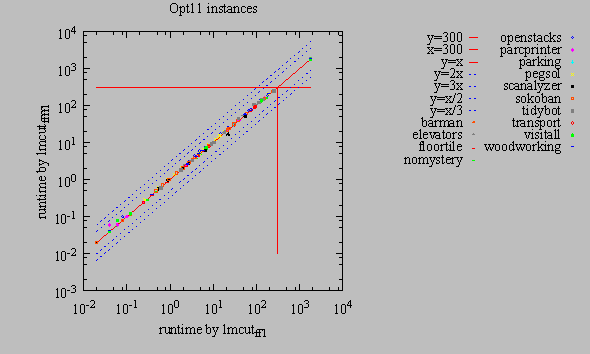
\includegraphics{tables/opt11-time-lmcut_ff-lmcut_ffff.pdf}
 \caption{Comparison of runtime on problems solved by both single FIFO search engine (ff) and a MultiSearch engine with 2 different instances of the same FIFO engine (ffff). The runtime difference was on average below a factor of x1.1, if we ignore the subsecond differences.}
 \label{ffff}
\end{figure}

This portfolio strategy has several interesting theoretical characteristics. First, if we ignore the negligeble cost of insertion and deletion to the open/closed list, we do not have to pay the extra cost evaluating the heuristic function for states $f<f^*$ thanks to the caching.
Recall that \astar always has to expand the states whose $f$ values are below $f^*$, the true distance from the initial state to the goal. If the heuristic estimate $h$, and in turn $f=g+h$ is the same, any tiebreaking strategy expands and evaluates the same set of nodes in $f<f*$.
Therefore, in region $f<f*$, our caching mechanism fully works and completely eliminates the possibility of extra evaluation caused by adding another queues.

Second, since the search terminates when \emph{some} engine finds a solution, and since the expansion happens in turns, the search effort within the final plateau is upper-bound by \emph{twice} the \emph{minimum} of the search efforts required by LIFO or FIFO engine. This is desirable because, as we saw in the last section, in some domains the gap between the best and worst tiebreaking strategy can be more than 10 times (Openstacks, for example).
When there are $n$ engines, then this increases to $n\times$ minimum amount of effort by each single engine.

Finally, we conducted experiments for evaluating our MultiSearch strategy.
% the number of evaluations and expansions, along with 
\refig{portfolio-ff} to \refig{portfolio-r} shows the runtime between different combinations of 2 or 3 tiebreaking strategies (FIFO+LIFO, FIFO+Random, LIFO+Random, FIFO+LIFO+Random) and the single tiebreaking strategies. The results support our claim that the evaluation never exceeds twice/thirds of the single search engine and, in practice, the evaluations are mostly the same with the single search engine, and in some domains with large plateaus, the search effort used by MultiSearch is more than ten times less than by the single strategy.

\begin{figure}[htbp]
 \centering
 \relsize{-2}
 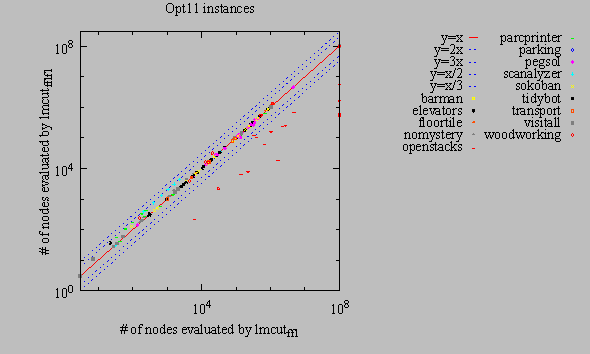
\includegraphics{tables/opt11-evaluated-lmcut_ff-lmcut_fflf.pdf}
 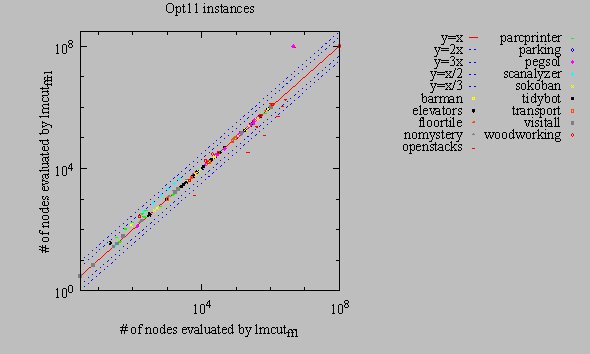
\includegraphics{tables/opt11-evaluated-lmcut_ff-lmcut_ffr.pdf}
 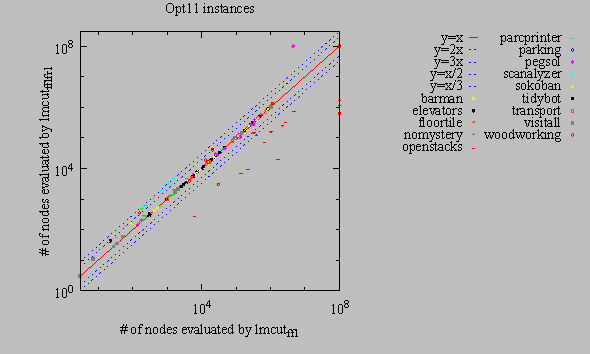
\includegraphics{tables/opt11-evaluated-lmcut_ff-lmcut_fflfr.pdf}
 \caption{}
 \label{portfolio-ff}
\end{figure}

\begin{figure}[htbp]
 \centering
 \relsize{-2}
 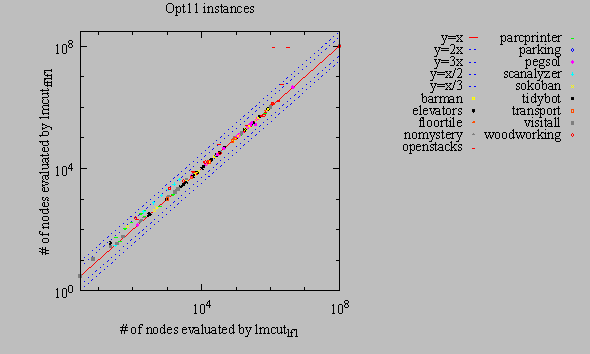
\includegraphics{tables/opt11-evaluated-lmcut_lf-lmcut_fflf.pdf}
 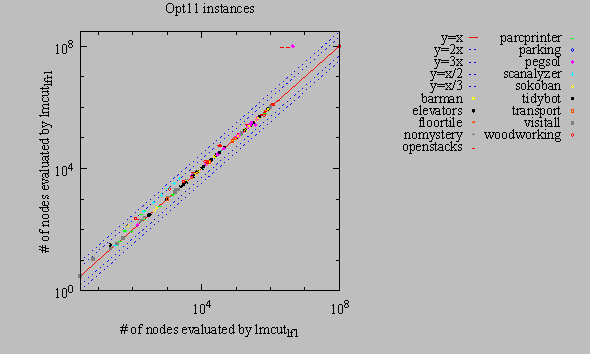
\includegraphics{tables/opt11-evaluated-lmcut_lf-lmcut_lfr.pdf}
 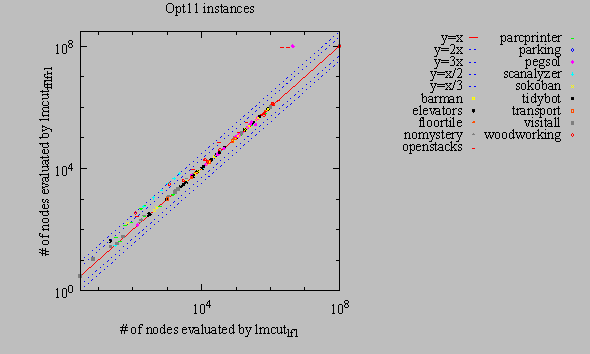
\includegraphics{tables/opt11-evaluated-lmcut_lf-lmcut_fflfr.pdf}
 \caption{}
 \label{portfolio-lf}
\end{figure}

\begin{figure}[htbp]
 \centering
 \relsize{-2}
 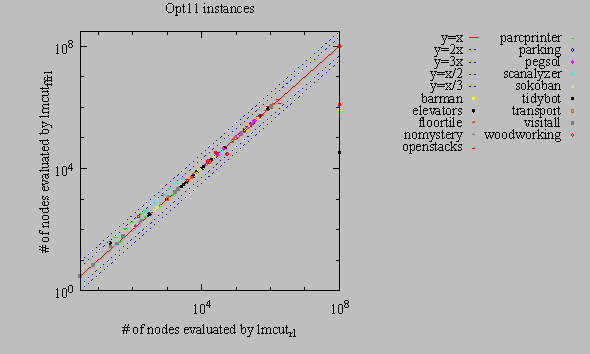
\includegraphics{tables/opt11-evaluated-lmcut_r-lmcut_ffr.pdf}
 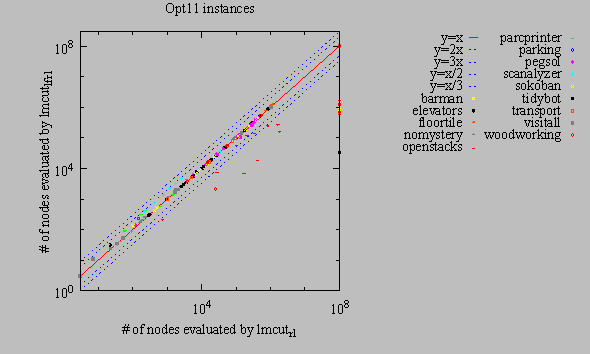
\includegraphics{tables/opt11-evaluated-lmcut_r-lmcut_lfr.pdf}
 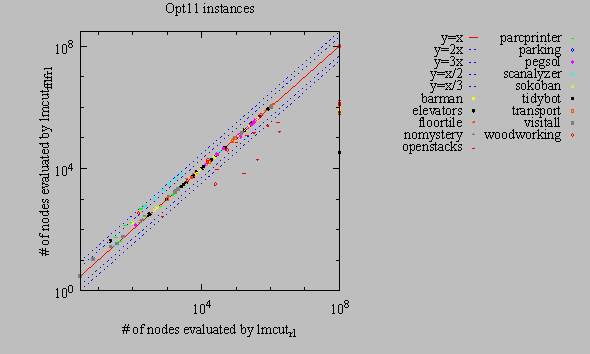
\includegraphics{tables/opt11-evaluated-lmcut_r-lmcut_fflfr.pdf}
 \caption{}
 \label{portfolio-r}
\end{figure}

